\documentclass[a4paper, 11pt]{article}
\usepackage{comment} % enables the use of multi-line comments (\ifx \fi)
\usepackage{lipsum} %This package just generates Lorem Ipsum filler text.
\usepackage{fullpage} % changes the margin
\usepackage[brazilian]{babel}
\usepackage{tabularx}
\usepackage[utf8]{inputenc}
\usepackage[T1]{fontenc}
\usepackage{graphicx}
\usepackage{indentfirst}
\usepackage[table]{xcolor}

\begin{document}
\noindent
\large\textbf{Melhoria de Processo de Software / Terceiro trabalho}\\
Lucas Albuquerque Medeiros de Moura \hfill 11/0015568 \\
Luciano Prestes Cavalcanti \hfill 11/0035208

\section*{Relatório Avaliação de Processo}

Este relatório visa descrever os resultados encontrados no processo de
desenvolvimento descrito no segundo trabalho da disciplina de Melhoria de
Processo de Software. O relatório irá abranger então uma breve descrição do
processo a ser analisado e seu contexto juntamente com a avaliação e melhoria
desse processo.

\section*{Processo Escolhido}\label{sec:processo}

O processo escolhido para receber a avaliação foi o processo usado pelo
Laboratório Avançado de Pesquisa e Produção de Software (LAPPIS) para o
desenvolvimento do software \textit{Noosfero}. Tal processo pode ser visto na
figura \ref{fig:processo_noosfero}

\begin{figure}[h]
  \centering
  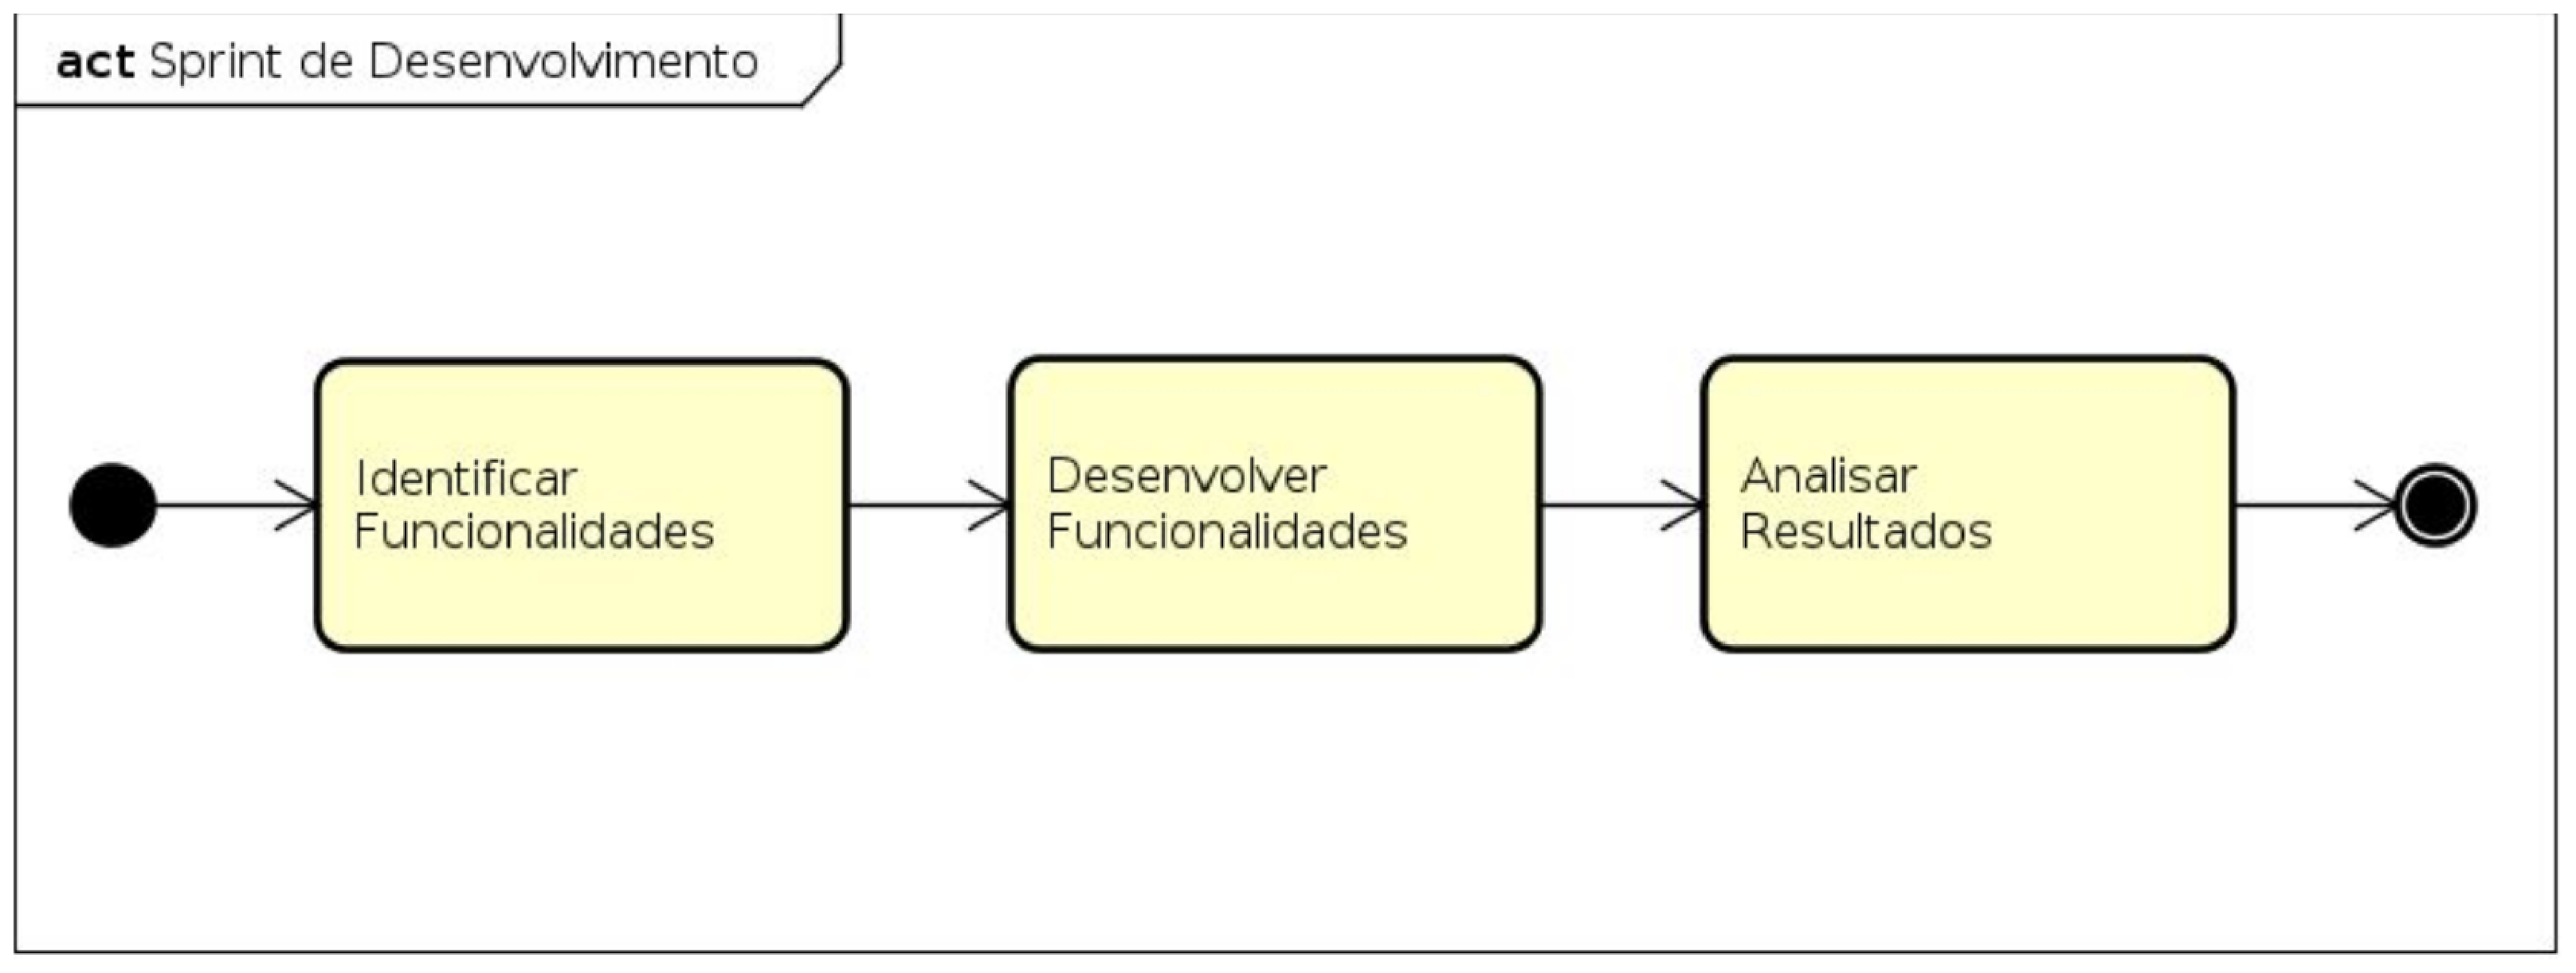
\includegraphics[width=0.9\textwidth]{figuras/processo_mps.eps}
  \caption{Processo de desenvolvimento para o software Noosfero}
  \label{fig:processo_noosfero}
\end{figure}

Tal processo é dividido em três fases distintas, sendo a primeira a fase de
identificar as funcionalidades. Tal fase tem como objetivo definir com a equipe
e o cliente o que será realizado durante uma \textit{sprint}. O processo para
essa fase pode ser visto na figura \ref{fig:processo_noosfero_funcionalidade}

\begin{figure}[h]
  \centering
  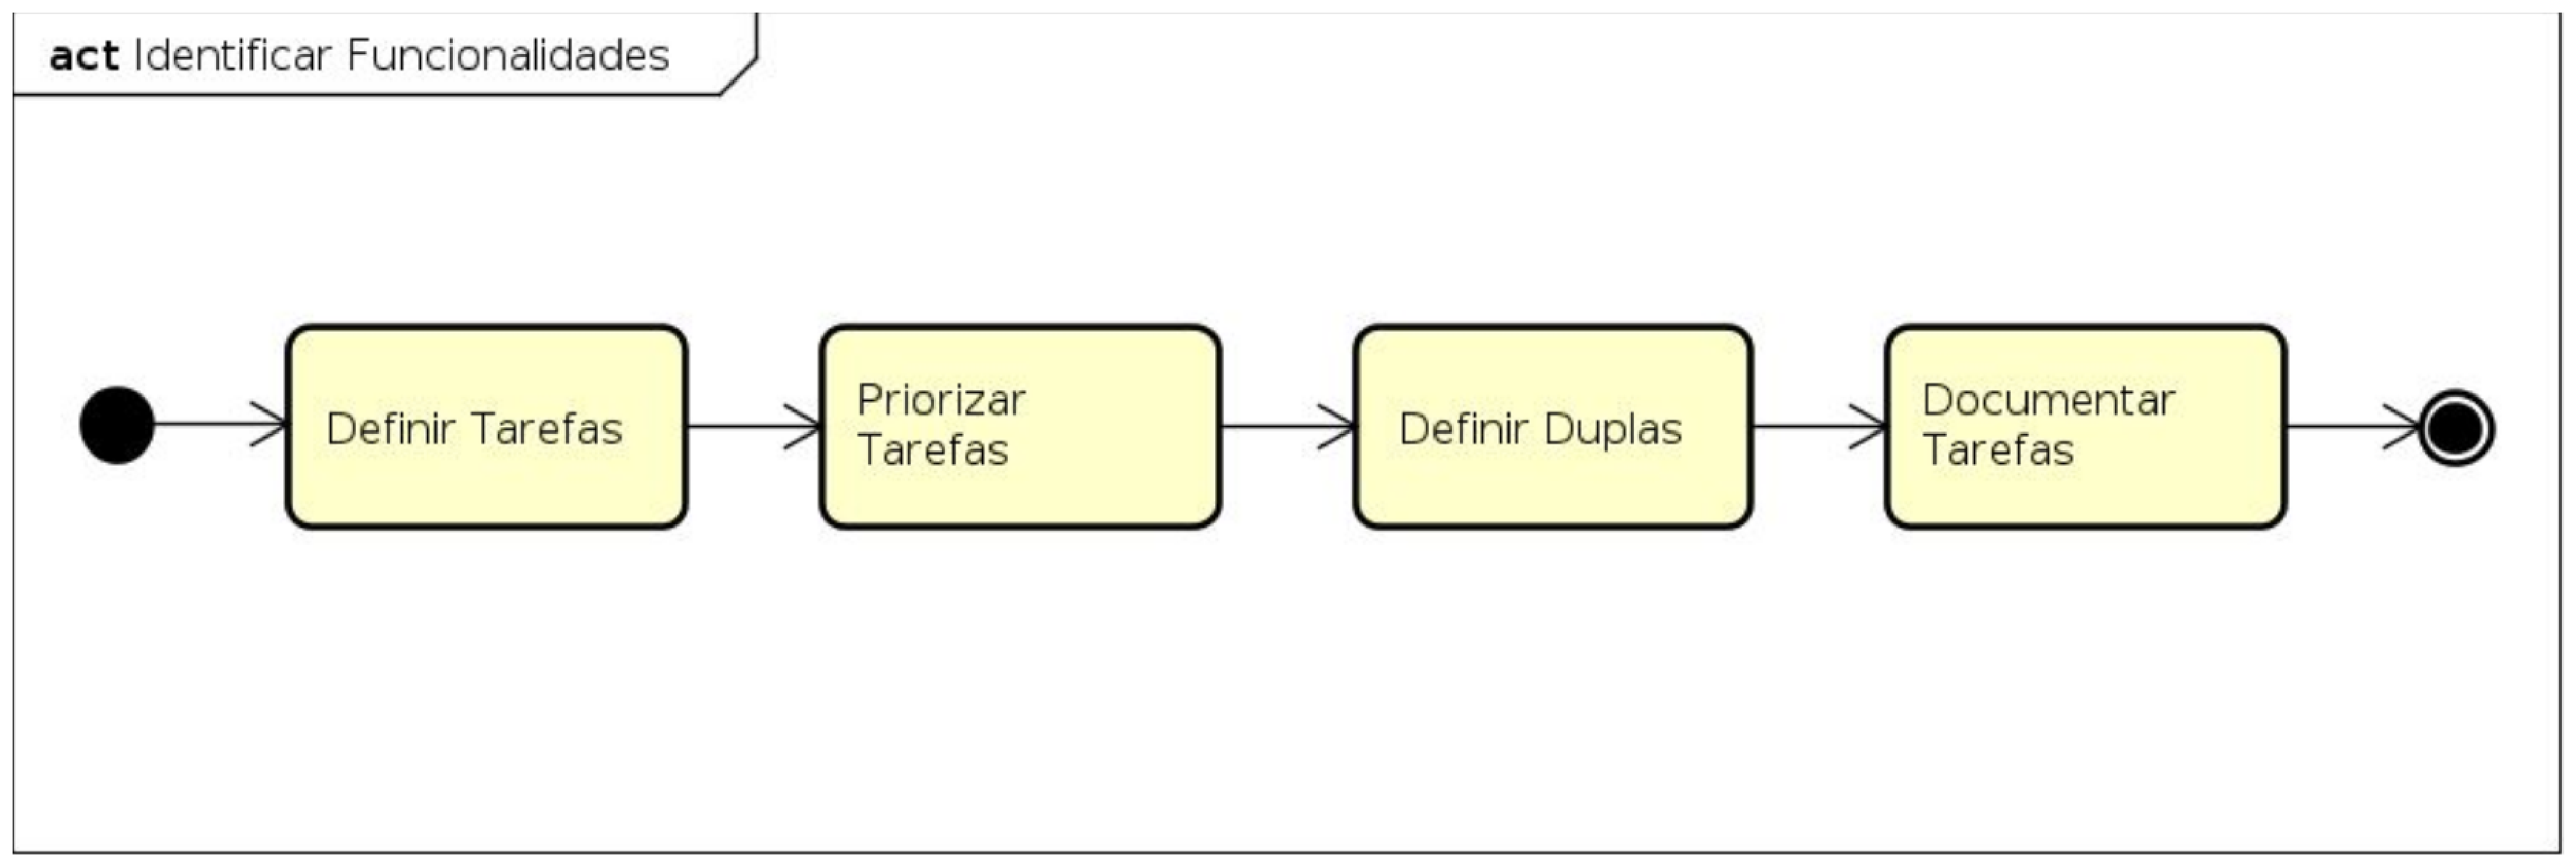
\includegraphics[width=0.9\textwidth]{figuras/processo_mps_funcionalidades.eps}
  \caption{Processo de identificar funcionalidades para o software Noosfero}
  \label{fig:processo_noosfero_funcionalidade}
\end{figure}

A segunda fase do processo é a desenvolver as funcionalides descritas na
primeira fase. As atividades de tal fase do processo podem ser vistas na figura
\ref{fig:processo_noosfero_desenvolvimento}

\begin{figure}[h]
  \centering
  \includegraphics[width=0.9\textwidth]{figuras/processo_mps_desenvolvimento.eps}
  \caption{Processo de desenvolver funcionalidades para o software Noosfero}
  \label{fig:processo_noosfero_desenvolvimento}
\end{figure}

Por fim, a última etapa do processo é a de reportar os resultados da sprint,
tanto em questão do que foi desenvolvido tanto sobre o que o time precisa
melhorar ou focar para próxima sprint. As atividades dessa fase do processo
podem ser vistas na figura \ref{fig:processo_noosfero_resultado}

\begin{figure}[h]
  \centering
  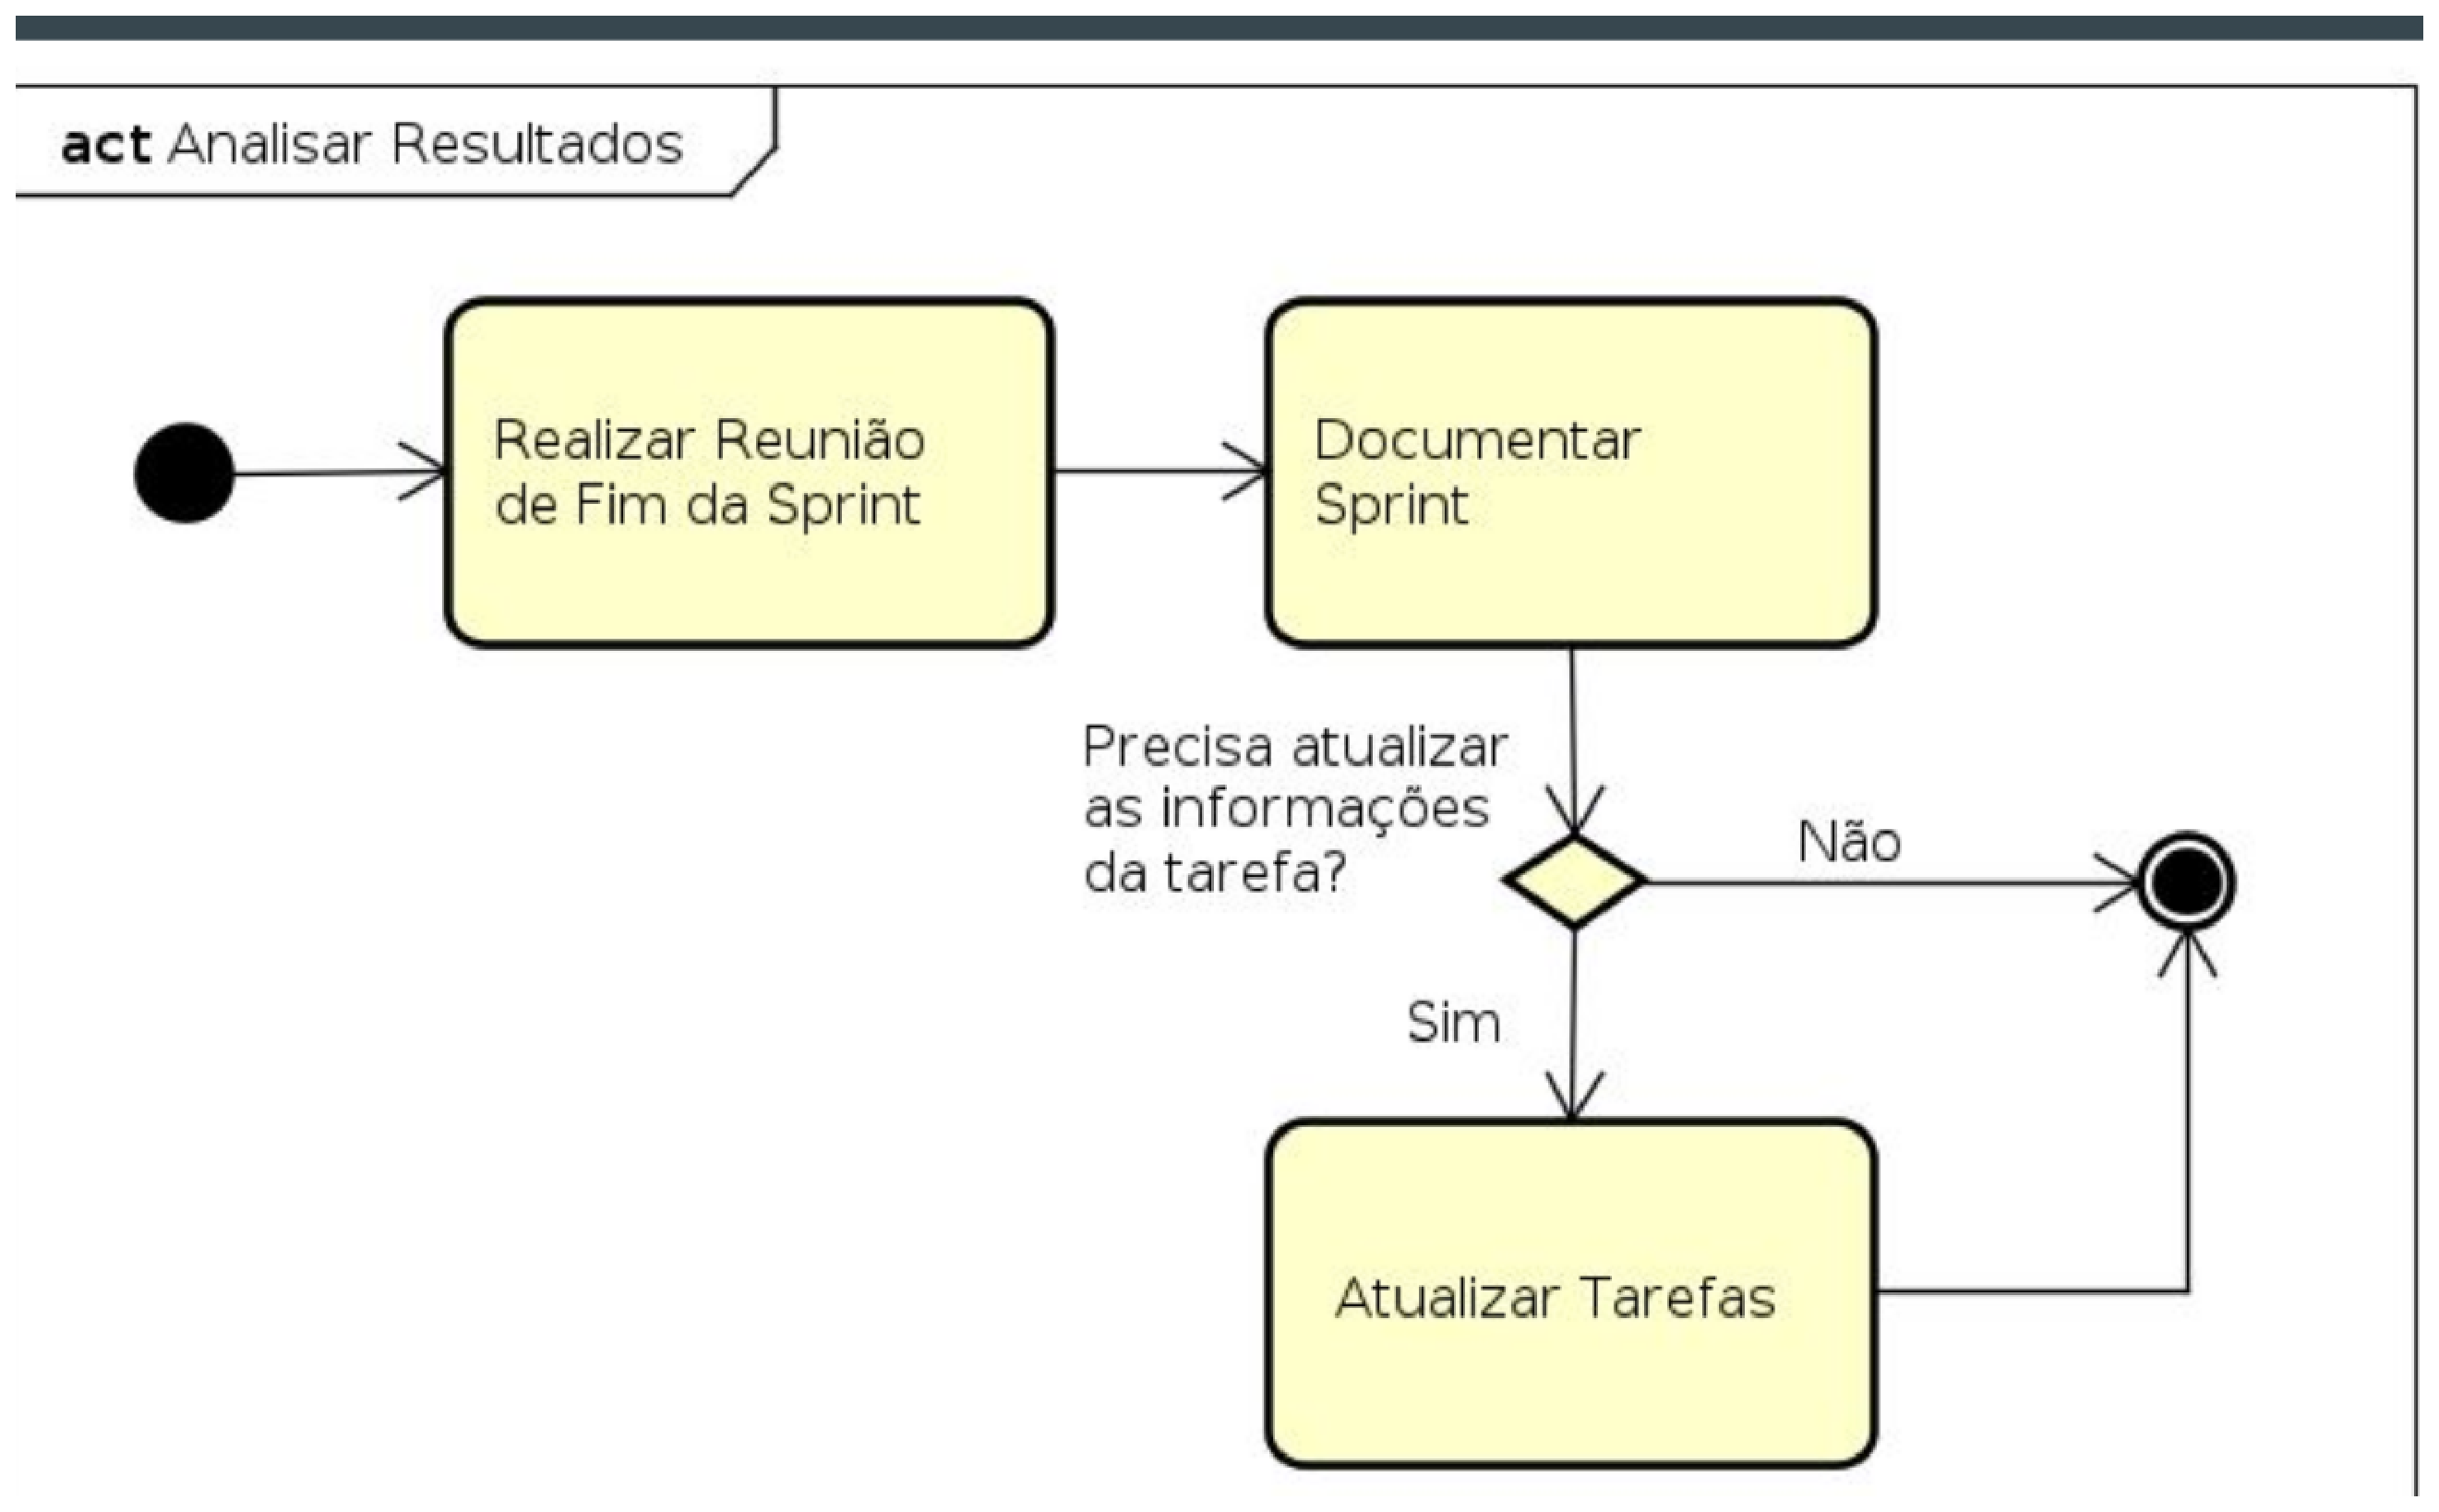
\includegraphics[width=0.9\textwidth]{figuras/processo_mps_resultados.eps}
  \caption{Processo de analisar resultados da sprint para o software Noosfero}
  \label{fig:processo_noosfero_resultado}
\end{figure}

\section*{Análise dos processos}

A análise do processo ocorrerá baseada na análise do MA-MPS.br, onde para
verificar se um processo está de fato implementado, deve-se observar por
evidências diretas e indiretas de que o processo está sendo seguido.

Uma evidência direta no caso dessa análise será o artefato que o processo se
propõe a fazer, já uma evidência indireta será dada por uma indicação que
membros do time saibam e realizam tais atividades.

A coleta de evidências direta será analisada pelos entregáveis gerados pelo
projeto. Já a coleta de evidência indireta será coletada prioritariamente por
observações durante o ciclo de trabalho.

Além disso, também seguirá em anexo a este trabalho, uma planilha com uma
análise mais geral sobre o processo, tratando de aspectos macros do mesmo.

Dito isso, as seções a seguir tratarão da análise de processo para cada um dos
subprocessos listados na seção \ref{sec:processo}.

\subsection*{Identificar necessidades}

Para as atividades deste subprocesso, pode-se ver a análise realizada na
seguinte tabela \ref{tab:necessidades}

\begin{table}[]
\centering
\caption{Análise do processo Identificar Necessidades}
\begin{tabularx}{\textwidth}{|X|X|X|X|}
\hline
Atividade & Evidência direta & Evidência indireta & Resultado \\ \hline
\multicolumn{1}{|l|}{Definir tarefas} & Documentação das issues a serem desenvolvidas no product backlog & Observou-se que o time sabe onde verificar tais tarefas e como cadastrar as mesmas & Atividade bem definida \\ \hline
\multicolumn{1}{|l|}{Priorizar tarefas} & As tarefas priorizadas são associadas a uma sprint na wiki do projeto & Pode-se observar que o time sabia onde buscar quais eram as tarefas da sprint & Atividade bem definida \\ \hline
\multicolumn{1}{|l|}{Definir duplas} & As duplas são associadas sempre em uma issue & As integrantes do time sabiam quem era suas duplas e caso tivessem faltado no dia, também sabiam onde verificar tal informação. & Atividade bem definida \\ \hline
\multicolumn{1}{|l|}{Documentar tarefas} & A documentação das tarefas é feita logo após a reunião e pode ser encontrada no repositório do projeto. & Alguns integrantes do time apenas usam o título da tarefa como documentação, o que pode ser ruim caso a tarefa se alongue. & Atividade parcialmente definida \\ \hline
\label{tab:necessidades}
\end{tabularx}
\end{table}

\subsection*{Desenvolver funcionalidades}

Para as atividades deste subprocesso, pode-se ver a análise realizada na
seguinte tabela \ref{tab:desenvolvimento}

\begin{table}[]
\centering
\caption{Análise do processo Desenvolver Funcionalidades}
\label{tab:desenvolvimento}
\begin{tabularx}{\textwidth}{|X|X|X|X|}
\hline
Atividade & Evidência direta & Evidência indireta & Resultado \\ \hline
Desenvolver solução & O código para uma solução sempre se encontra em uma branch do repositório do projeto. & Observou-se que algumas vezes membros do time esquecem de mandar seu código ao fim do dia para o repositório, deixando as modificações salvas apenas em seu ambiente local. & Atividade parcialmente definida. \\ \hline
Atualizar tarefa & Algumas tarefas não são atualizadas no ferramenta gitlab, & Percebeu-se que muitos dos membros do time se esquecem de atualizar o andamento de uma tarefa. & Atividade parcialmente definida. \\ \hline
Solicitar revisão & Sempre que uma modificação deve ser feita, a mesma tem que passar por um processo de revisão. Isso pode ser observado no repositório do projeto por meio de merge requests. & Os integrantes do time sabem como funciona tal processo e como abrir uma requisição de revisão. & Atividade bem definida \\ \hline
Relatar status da tarefa & Ao término de uma sprint, as tarefas não concluídas devem ser atualizadas. Entretanto, foi possível encontrar tarefas que não atendiam esse objetivo. & Percebeu-se que alguns integrantes do time esqueceram de atualizar o status da tarefa ao término da sprint. & Atividade parcialmente definida \\ \hline
\end{tabularx}
\end{table}


\subsection*{Analisar resultados}

Para as atividades deste subprocesso, pode-se ver a análise realizada na
seguinte tabela \ref{tab:analisar}

\begin{table}[]
\centering
\caption{Análise do processo Analisar resultados}
\label{tab:analisar}
\begin{tabularx}{\textwidth}{|X|X|X|X|}
\hline
Atividade & Evidência direta & Evidência indireta & Resultado \\ \hline
Realizar reunião de fim de sprint & O time se reúne ao término da sprint para discutir o que foi feito & Todo o time sabe quando essa reunião ocorre e a importância de estar presente. & Atividade bem definida. \\ \hline
Documentar sprint & A documentação que reflete o que foi realizado na sprint se encontra sempre na wki do projeto. & Percebeu-se que o time sabe informar onde se encontra a documentação de sprints passadas. & Atividade bem definida. \\ \hline
Atualizar tarefas & Ao término da sprint as tarefas não concluídas voltam para o backlog & Percebeu-se que o time entende como fazer uma tarefa voltar para o backlog e o porque disso acontecer. & Atividade bem definida \\ \hline
\end{tabularx}
\end{table}

\section*{Análise dos resultados}

\begin{table}[h]
\centering
\resizebox{\textwidth}{!}{\begin{tabular}{|l|l|l|l|l|}
\hline

\rowcolor[HTML]{EFEFEF}
\multicolumn{2}{|c|}{\textbf{Processo Avaliado}} &
\multicolumn{2}{|c|}{} \\ \hline

\rowcolor[HTML]{EFEFEF}
{\textbf{Requerido/Melhoria}} & {\textbf{Resultado Esperado}} &
{\textbf{Problema}} & {\textbf{Sugestão para Corrigir}} \\ \hline

\end{tabular}}
\caption{Relatório de Avaliação}
\label{tab:relatorio_de_avaliacao}
\end{table}

\end{document}
